\section{Method}
\subsection{Participants}
The study has been approved by the PaLS - Institute of Cognitive Neuroscience/ BUCNI LREC as Project ID 0210. For the acquaintance group, 17 interconnected participants who provided their laughter recordings in 2012 were contacted again, and 10 of them responded and completed the experiment. Seven additional family members/friends of these laughers were recruited through a snowball sampling technique (referred by laughers). The final acquaintance group of 17 participants consisted of 10 females and 7 males, between the ages of 18 and 61 (\textit{M }= 41.29, \textit{SD} = 16.81).

\subsection{Materials}
The experiment was built and conducted on the Gorilla (https://gorilla.sc/), an online experiment builder platform \citep {anwyl2020gorilla}. Participants completed the task on their personal computers and headphones.

\subsubsection{Laughter Perception Task (LPT)}

LPT consisted of two blocks. Both blocks involved listening to recordings of laughter. 68 spontaneous laughter recordings were collected from 17 laughers (7 females and 10 males) in 2012. While these participants were shown funny YouTube videos, their natural responses were recorded in an Anechoic chamber. Each laugher contributed two recordings per block.

In Block 1, participants were not informed of the names of laughers in the recording. After listening to each recording, they were asked to 1) rate the contagion (“How much does this laughter make you laugh”) on a scale from 1, meaning “I don’t want to laugh at all,” to 10 “I laugh a lot.” 2) rate the familiarity (“does this laughter sound familiar?”) on a scale from 1, meaning “not familiar,” to 10, “very familiar” (Figure 1). In order to ensure participants focused on the task, three vigilance trials were also applied in random order, in which participants were asked to select the number that the speaker in the audio said. A total of 37 trials ( 34 laughter perception trials and 3 vigilance trials) were conducted.

In Block 2, before listening to the laughter recording, participants in the acquaintance group were presented with the laugher’s name, a manipulation reffered to as the informing effect. After listening to each recording, they were again asked to rate the contagiousness of laughter on the same scale as above. Differently, this time, they were asked to judge their closeness with the laugher (“Is this person close to you?”) instead of familiarity, on a scale from 1 “not close” to 10 “very close” (see Figure~\ref{fig1}). Three vigilance trials were applied. A total of 37 trials ( 34 laughter perception trials and 3 vigilance trials) were conducted.

\begin{figure}[h!] 
\centering
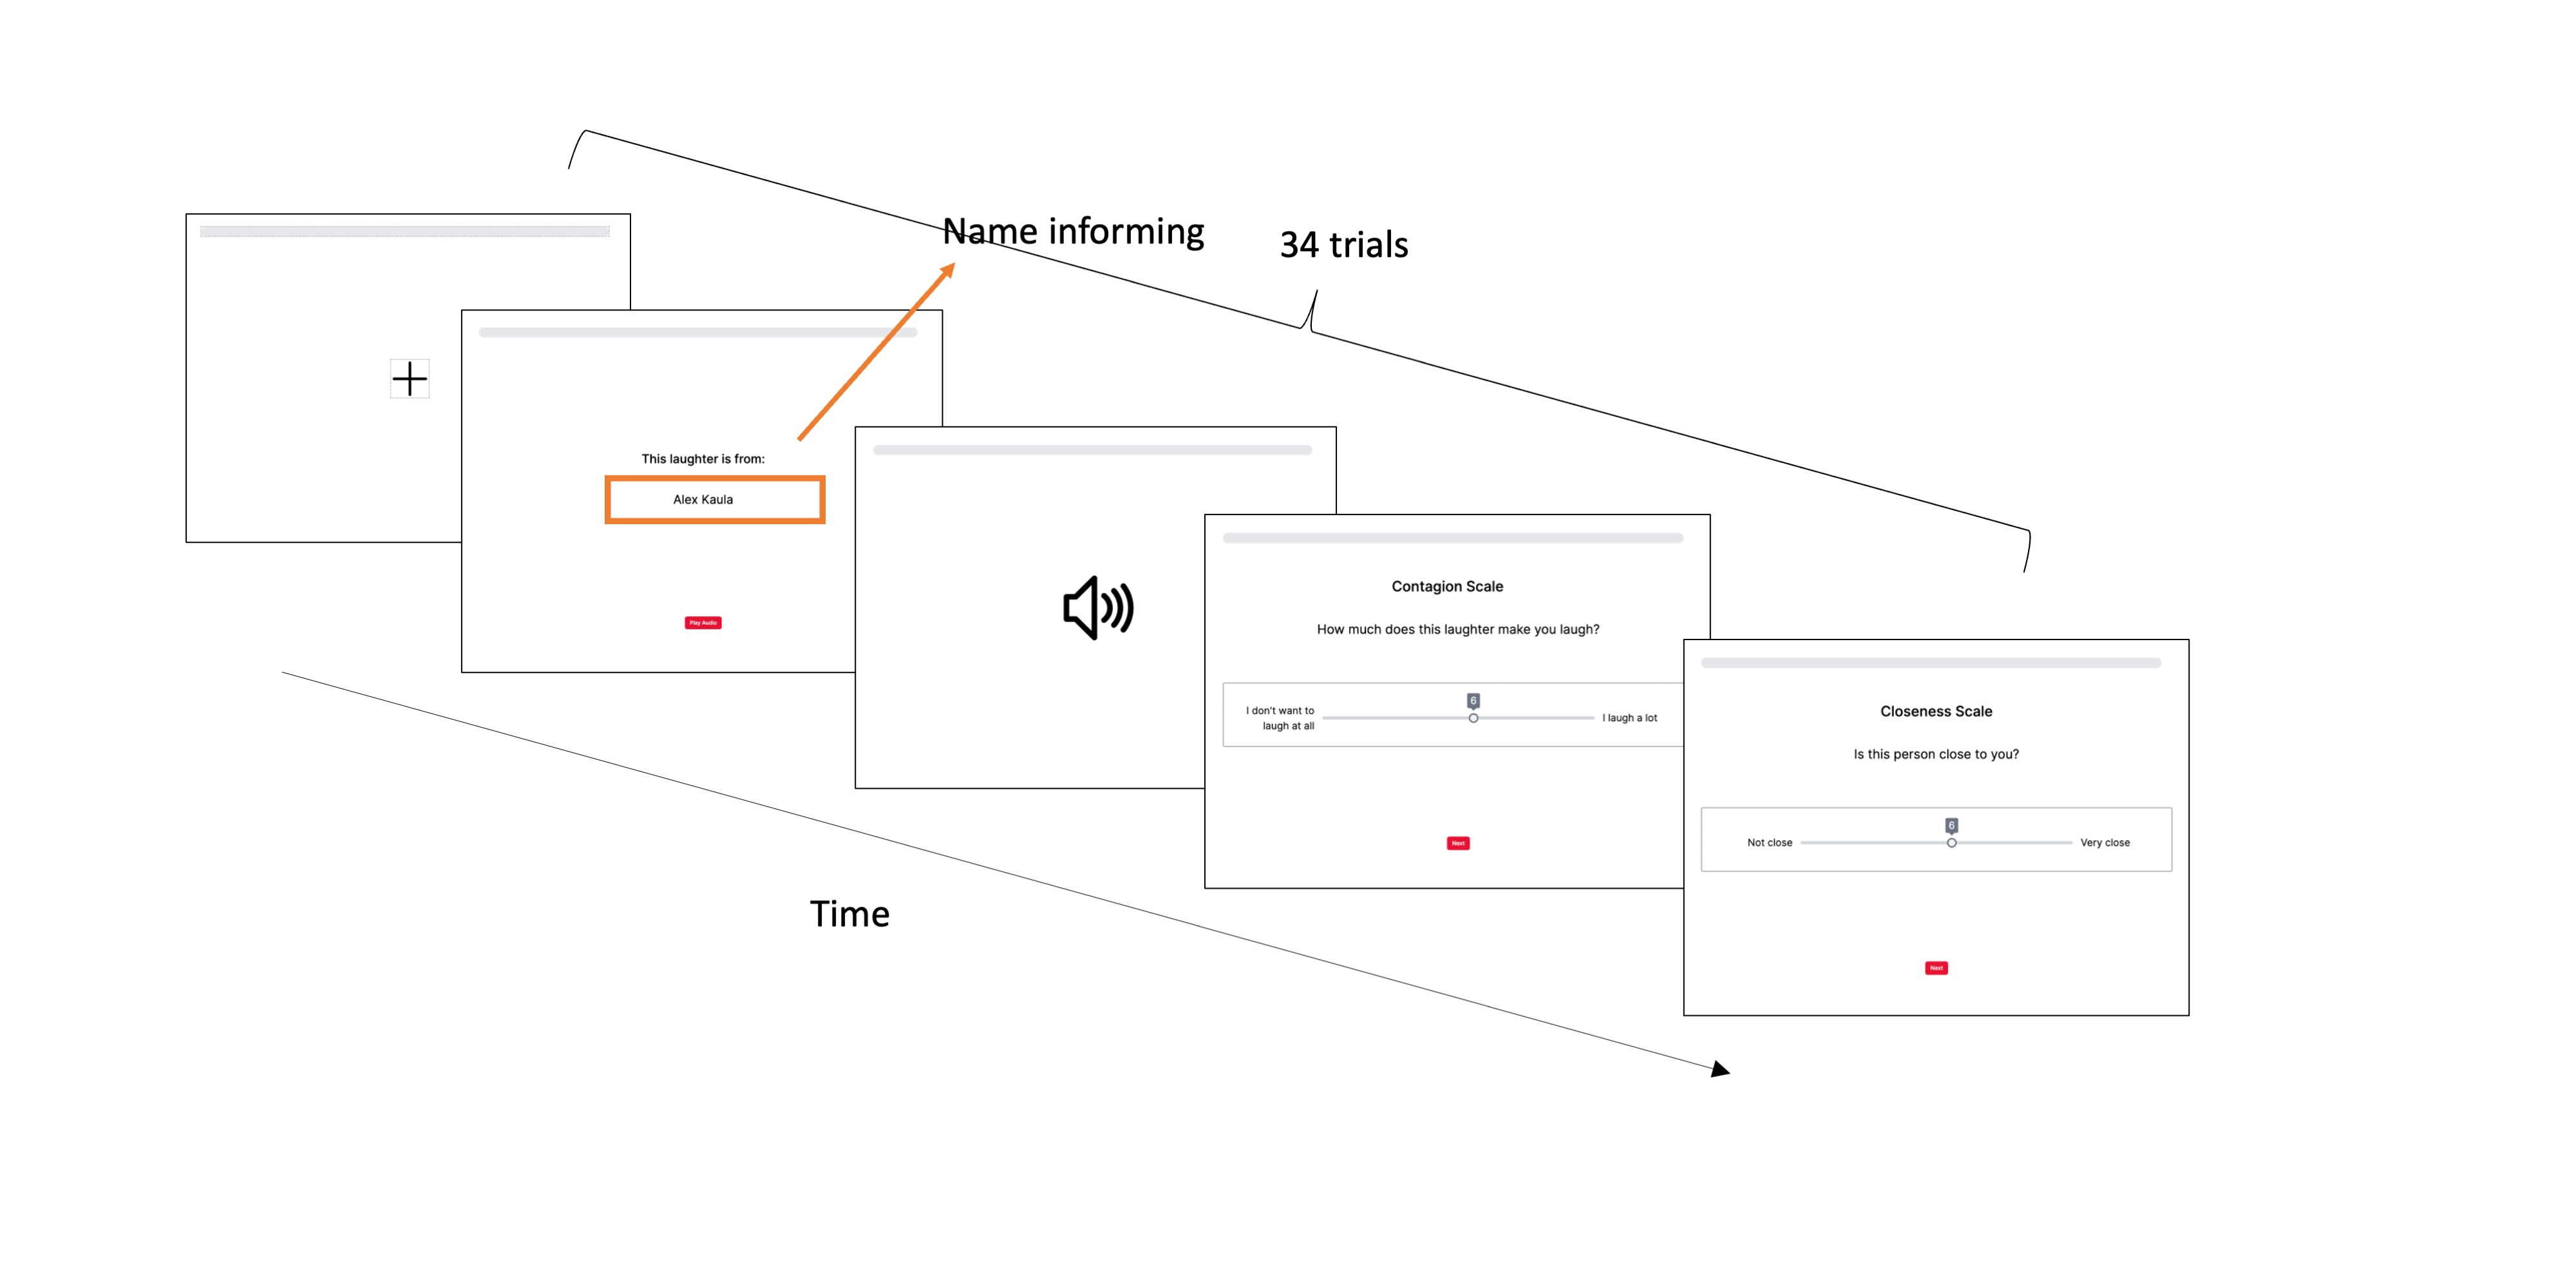
\includegraphics[width=1\textwidth]{Slide2.jpeg}
\caption{\label{fig1}Laughter Perception Block 1 Illustration.}
\end{figure}

In Block 2, before listening to the laughter recording, participants in the acquaintance group were presented with the laugher’s name, a manipulation referred to as the informing effect. After listening to each recording, they were again asked to rate the contagiousness of laughter on the same scale as above. Differently, this time, they were asked to judge their closeness with the laugher (“Is this person close to you?”) instead of familiarity, on a scale from 1 “not close” to 10 “very close”(Figure ~\ref{fig2}). Three vigilance trials were applied. A total of 37 trials ( 34 laughter perception trials and 3 vigilance trials) were conducted.

The stranger group received the same task format as Block 1. As we assumed participants from the stranger group may not personally know the laughers in the recordings, providing the laughers’ names would not affect their performance in general, and therefore, there was no name-informing procedure for the stranger group in Block 2.

\begin{figure}[h!] 
\centering
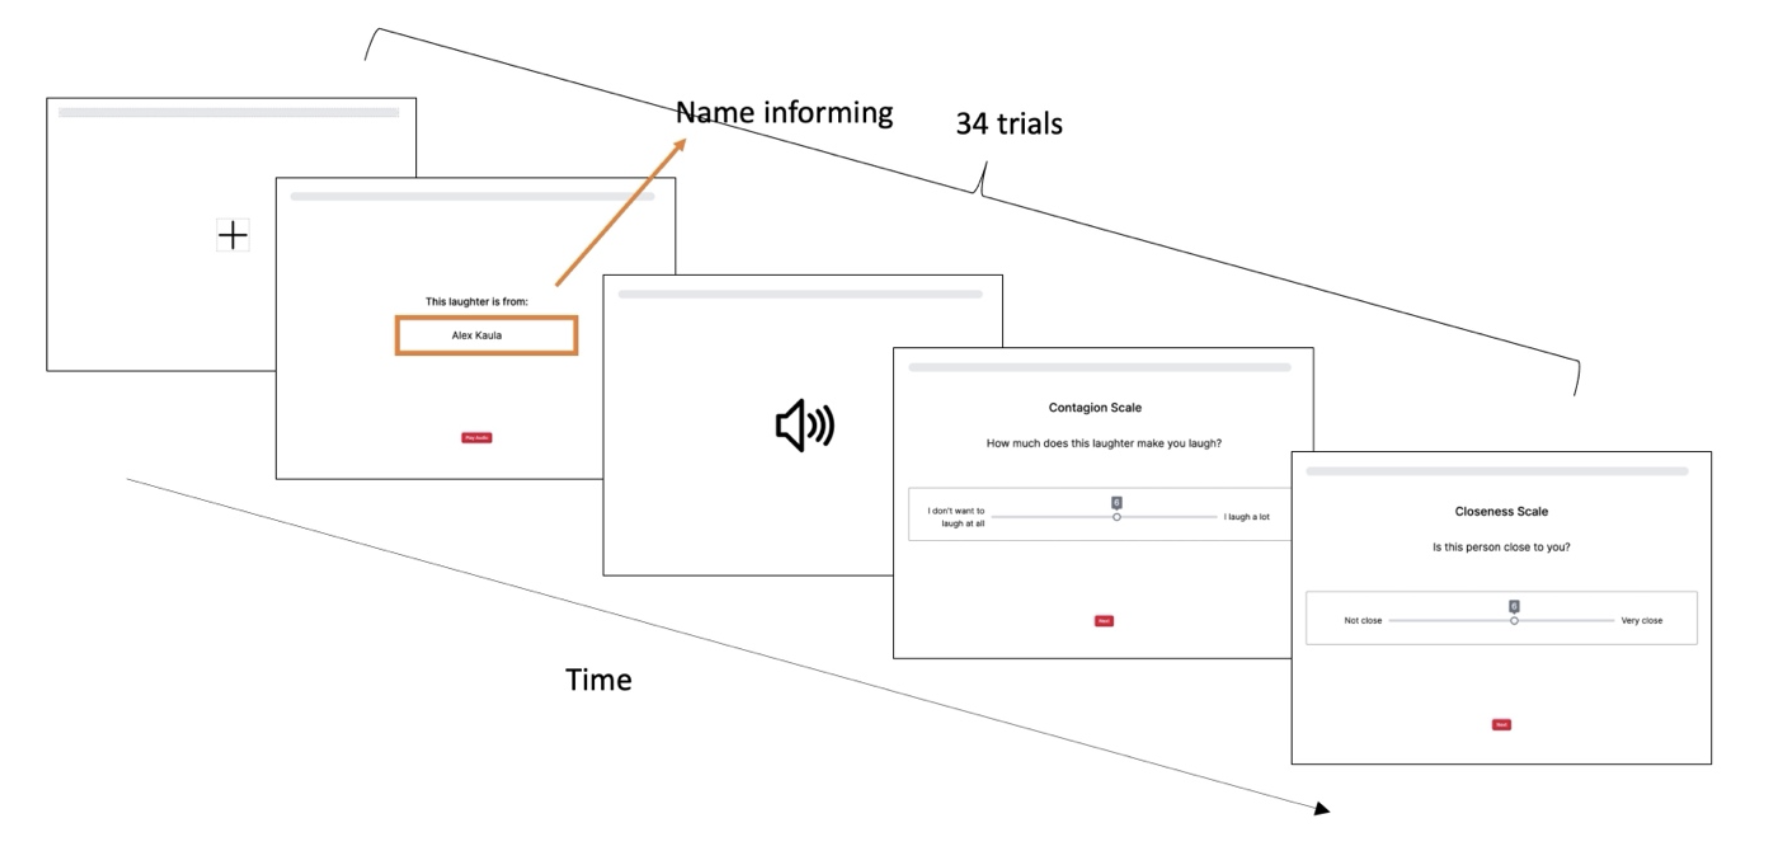
\includegraphics[width=13cm]{Screenshot 2025-09-03 at 11.29.56.png}
\caption{\label{fig2}Laughter Perception Block 2 Illustration.}
\end{figure}


\subsection{Procedure}
Participants in the acquaintance group were invited to the Gorilla online experiment through an email link; the stranger group was invited through Prolific. After providing informed consent, participants completed a sound check to ensure the audio devices were connected.

Participants were first asked to provide demographic information (age, gender, sex) and then completed two questionnaires (LSAS and LPPQ).

\subsection{Statistical analyses}
 For the primary research question (H1 – H3), we were interested in the effect of social connectedness on laughter contagion at different manipulations. Only data from acquaintance groups (\textit{n} = 17) were used, as we assume that the stranger group does not experience social effects. To account for variations within individuals and items, we built a Linear Mixed-effects Model using the lmer function from the lmer4 package (Bates et al., 2015) in R (version 4.4.1). Fixed effects consisted of the social connectedness effect, informing effect, and their interaction. For random effects, we started with the maximal structure with the item and the participant intercepts and slopes (Barr et al., 2013), but not all models converge with this structure. In order to ensure the model converges, we selected a maximal random structure that consisted of by-participants (ID) random slopes and intercepts and by-item intercepts only. This random effect structure accounted for individual differences (individual propensity to laughter contagion and fixed effects) and item differences (variations in contagion level across each laughter recording). Overall, the use of a Linear Mixed-effects Model allowed us to assess the impact of the predictor and manipulation on changes in the outcome variables. The estimates in the mixed-effects model represented the estimated effect size. Statistical significance was set at p <0.05. 
